\section{Chl-Kataboliten des Brokkoliblattes mithilfe von LC-MS identifiziert} \label{sec:ChlKatabolitenBrokkoli}

Das HPLC Chromatogramm in Abbildung \ref{fig:HPLCChromatogramm} zeigt, welche der Kataboliten mithilfe ihrer UV/Vis Spektren eindeutig identifiziert werden konnten. Es dürfte sich dabei ob ihrer etwas höheren Intensitäten um die Hauptkataboliten des Brokkoliblattes handeln. Dies müsste jedoch in gezielten quantitativen Messungen weiter und genauer untersucht werden.

\begin{figure}[!htbp]
  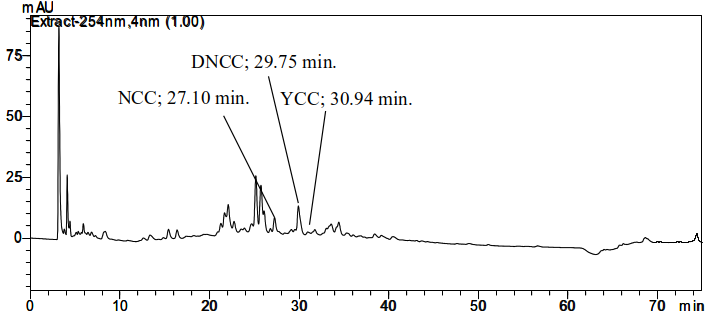
\includegraphics[width=\textwidth]{figures/Kapitel6/keineReaktion/VWA_HPLC_Chromatogramm_keineReaktion.png}
  \caption[HPLC Chromatogramm vor der Reaktion, Quelle: Autor]{\gls{hplc} Chromatogramm - die hervorgehobenen Peaks entsprechen den Retentionszeiten und der Art der \gls{Chl-K}en, die über ein Online-UV/Vis Spektrum bestimmt wurden; gefunden wurden ein \gls{NCC} bei 27.10 min. (Abbildung \ref{fig:NCC2725}), ein DNCC bei 29.75 min. (Abbildung \ref{fig:DNCC2991}) und ein YCC bei 30.94 min. (Abbildung \ref{fig:YCC3094})}
  \label{fig:HPLCChromatogramm}
\end{figure}

\begin{figure}[!htbp]
  \centering
  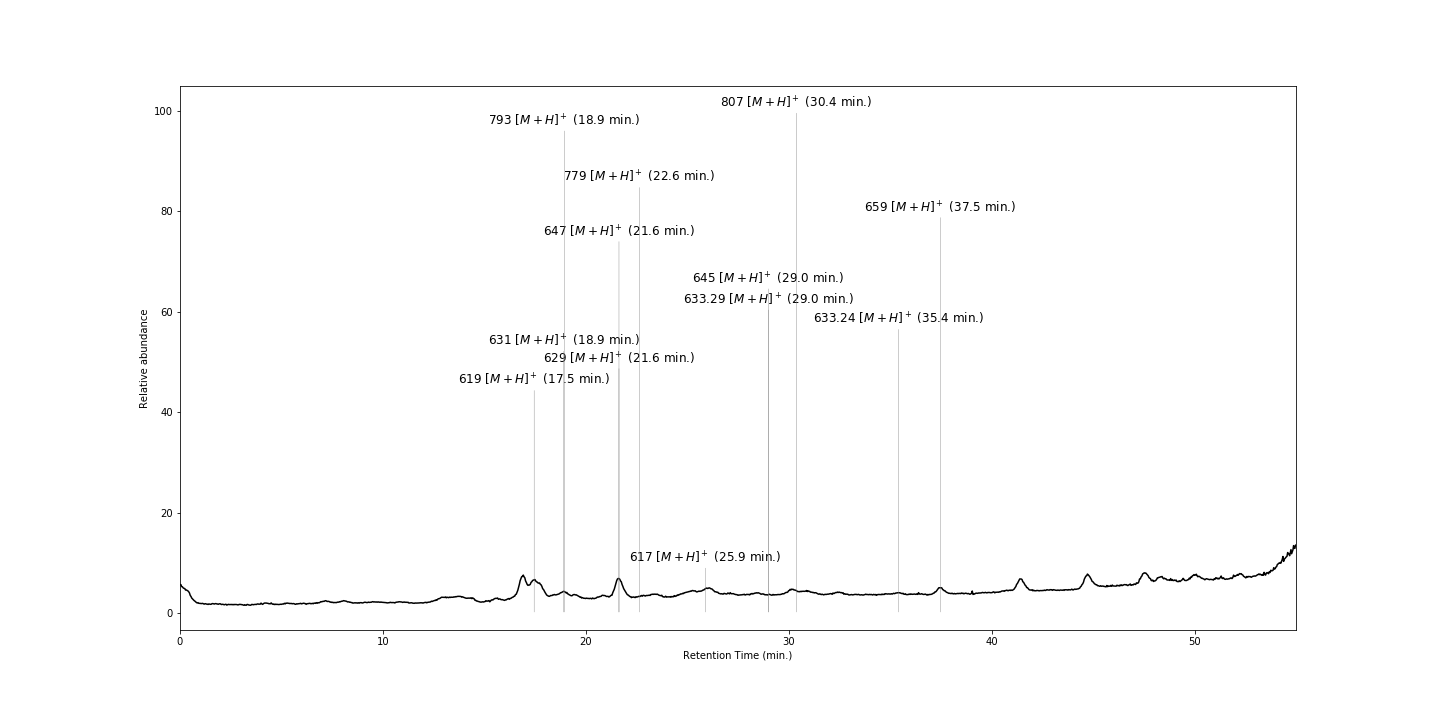
\includegraphics[width=1.4\textwidth, center]{figures/Kapitel6/keineReaktion/Kuerbis_Analyse_keineReaktion2_Ganzes_Spektrum.png}
  \caption[LC-MS Chromatogramm vor der Reaktion, Quelle: Autor]{\gls{lcms} Chromatogramm}
  \label{fig:LCMSChromatogramm}
\end{figure}

Mit dem Massenspektrometer wurden die in Tabelle \ref{tab:LCMSKataboliten} aufgelisteten Phyllobiline identifiziert. In dieser Tabelle werden neben den Summenformeln auch die exakten Molekülmassen (in Da), die Art des \gls{Chl-K} (NCC, DNCC, YCC, DYCC) und die Retentionszeit in der \gls{hplc} (soweit eindeutig feststellbar) angegeben. \\

Eine so große Anzahl an \gls{Chl-K}en wie in Tabelle \ref{tab:LCMSKataboliten} vorzufinden wäre ungewöhnlich. Bei einer Betrachtung der Summenformeln und exakten Molekülmassen fällt jedoch auf, dass sich einige \gls{Chl-K}en um genau ein C-Atom und zwei H-Atome unterscheiden (entsprich einem Massenunterschied von 14 Da). 

Da alle identifizierten \gls{Chl-K} eine freie Carbonsäuregruppe an Position 8\textsuperscript{2} besitzen, wird angenommen, dass diese bei der Aufarbeitung der Probe mit \gls{meoh} (Kapitel \ref{sec:HPLCAufarbeitungderProbe}) mit diesem reagieren und einen Methylester ausbilden. In der Spalte Herkunft (abgekürzt mit H.) der Tabelle \ref{tab:LCMSKataboliten} wird demnach festgehalten, von welchem \gls{Chl-K}en die jeweilige Verbindung stammt. Es handelt sich dabei also um keine \gls{Chl-K}en, sondern nur um deren Reaktionsprodukte mit \gls{meoh}. In der \gls{hplc} konnten sie jedoch nicht identifiziert werden. \\

\begin{table*}\centering
  \ra{1.3}

  \begin{tabular}{cccccc}\toprule
 Bezeichnung & Summenformel & M (in Da) & Typ & RT\textsubscript{HPLC} (in min.) & H. \\
\midrule
\rowcolor{black!20} Bo-DYCC & \ch{C33H37O8N4} & 617.2635 & DYCC & 30.94? & - \\
 Bo-DNCC & \ch{C33H39O8N4} & 619.2793 & DNCC & 26.72 & - \\ 
\rowcolor{black!20} • & \ch{C34H37O8N4} & 629.2639 & • & - & - \\ 
 - & \ch{C34H39O8N4} & 631.2795 & DYCC & 29.91, 30.94 & Bo-DYCC \\ 
\rowcolor{black!20} - & \ch{C34H41O8N4} & 633.2955 & DNCC & - & Bo-DNCC \\ 
 • & \ch{C36H33O7N4} & 633.2339 & • & • & - \\ 
\rowcolor{black!20} Bo-YCC & \ch{C34H37O9N4} & 645.2593 & YCC & - & - \\ 
 Bo-NCC-3 & \ch{C34H39O9N4} & 647.2748 & NCC & 33.04 & - \\ 
\rowcolor{black!20} - & \ch{C35H39O9N4} & 659.2741 & YCC & - & Bo-YCC \\
 Bo-DNCC-2 & \ch{C39H47O13N4} & 779.3181 & DNCC & • & - \\ 
\rowcolor{black!20}Bo-NCC-1 & \ch{C40H49O13N4} & 793.3336 & NCC & 29.91 & - \\ 
 - & \ch{C41H51O13N4} & 807.3491 & NCC & - & Bo-NCC-1 \\ 
\bottomrule
  \end{tabular}
  \caption[Übersicht über die Chl-Kataboliten des Brokkoliblattes, Quelle: Autor]{Übersicht über die gefundenen Chl-Kataboliten des Brokkoliblattes und ihren Methylestern, die sich aus der Reaktion der freien Carbonsäure mit \gls{meoh} ergeben (die Summenformeln und die exakten Molekülmassen beziehen sich auf die [M+H]\textsuperscript{+} Ionen)}
  \label{tab:LCMSKataboliten}
\end{table*}

Bei einer Retentionszeit von 27.10 min. konnte über Online-UV/Vis ein \gls{NCC} (Abbildung \ref{fig:NCC2725}) identifiziert werden, da er bei einer Wellenlänge von 315 nm eine charakteristische Bande aufweist. Der von den Retentionszeiten dazugehörige \gls{Chl-K} im Massenspektrum wäre der Bo-DNCC (mit einer Retentionszeit von 17.5 min im Massenspektrometer - Abbildung \ref{fig:LCMSChromatogramm}). Bei diesem handelt es sich jedoch um einen \gls{DNCC}. Es wurde versucht, das unlogische Ergebnis durch Überlagerungen mehrer \gls{Chl-K}en zu erklären, was aber nicht möglich war (Abbildung \ref{fig:LCMSChromatogrammAufspaltung}). Es bleibt somit das Zustandekommen dieses UV/Vis Spektrums ungeklärt. 

Bei einer Retentionszeit von 29.75 min. konnte ein UV/Vis Spektrum eines \gls{DNCC}s (Abbildung \ref{fig:DNCC2991}) aufgenommen werden. Nach den Retentionszeiten im Massenspektrometer (Abbildung \ref{fig:LCMSChromatogramm}) kann diesem UV/Vis Spektrum der \gls{Chl-K} Bo-NCC-1 zugeordnet werden. Auch der Methylester des Bo-YDNCC ist zu dieser Retentionszeit im Massenspektrometer vorzufinden und trägt damit vermutlich zur Entstehung des Signals bei, was die Verzerrungen bewirken könnte (Abbildung \ref{fig:LCMSChromatogrammAufspaltung}).

\begin{figure}[!htbp]
  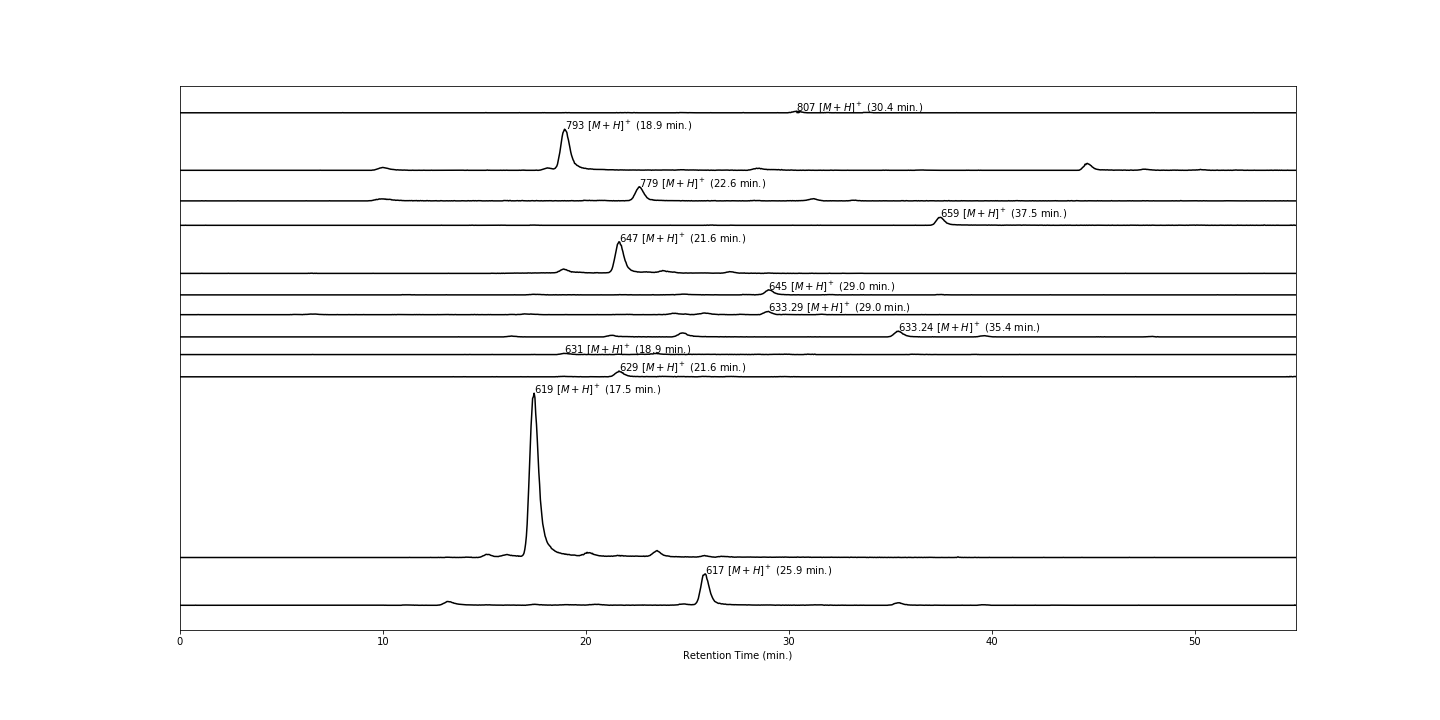
\includegraphics[width=1.4\textwidth, center]{figures/Kapitel6/keineReaktion/Kuerbis_Analyse_keineReaktion2_LC-ESI-MS.png}
  \caption[LC-MS Chromatogramm vor der Reaktion - Aufspaltung der Signale, Quelle: Autor]{\gls{lcms} Chromatogramm zur besseren Darstellung von Überlagerungen von Chlorophyllkataboliten, um diverse unlogische Schlüsse besser verstehen zu können}
  \label{fig:LCMSChromatogrammAufspaltung}
\end{figure}

Bei einer Retentionszeit von 30.94 min. ist das UV/Vis Spektrum charakteristisch für einen \gls{YCC} (Abbildung \ref{fig:DNCC2991}). Im Massenspektrometer wurde zu dieser Retentionszeit der Methylester des Bo-YDNCC gefunden (bei einer Retentionszeit von 18.9 min). Auch hier lässt sich keine Verbindung finden, bei der die Retentionszeiten von \gls{hplc} und Massenspektrometer exakt zusammenpassen. Es könnte auch hier wieder zu einer Überlagerung kommen (vielleicht mit dem Bo-YDNCC). Diese Überlagerungen könnten durch Isomere der einzelnen \gls{Chl-K}en bedingt sein. \\
 

Um das Zustandekommen der nicht identifizierbaren UV/Vis Spektren zu erklären wurden Diagramme wie in Abbildung \ref{fig:LCMSChromatogrammAufspaltung} erstellt. Es handelt sich dabei um ein Chromatogramm jedes einzelnen im Massenspektrometer während eines \gls{lcms} Laufes identifizierten \gls{Chl-K}en. Die Intensitäten wurden auf den höchsten im Zeitraum vorkommenden Peak skaliert. Bei den gekennzeichneten Peaks handelt es sich um jene, bei denen die jeweilige Verbindung die höchste Intensität im Chromatogramm zeigte. Peaks etwaiger Stereoisomere werden nicht beachtet. Mithilfe dieser Abbildung sollten etwaige Überlagerungen ersichtlich werden. 

\begin{figure}[!htbp]
  \begin{subfigure}[b]{0.5\textwidth}
    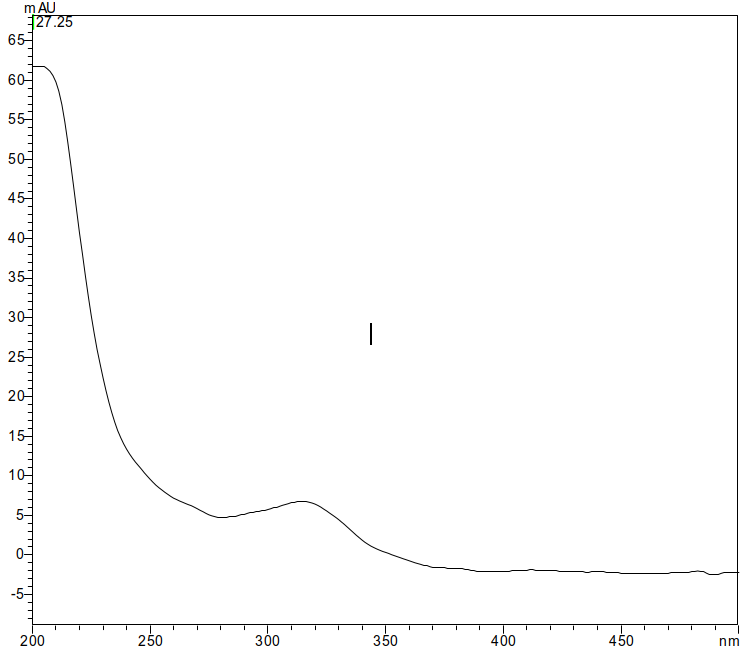
\includegraphics[width=\textwidth]{figures/Kapitel6/keineReaktion/NCC2725.png}
    \caption{}
    \label{fig:NCC2725}
  \end{subfigure}
  \hfill
  \begin{subfigure}[b]{0.5\textwidth}
    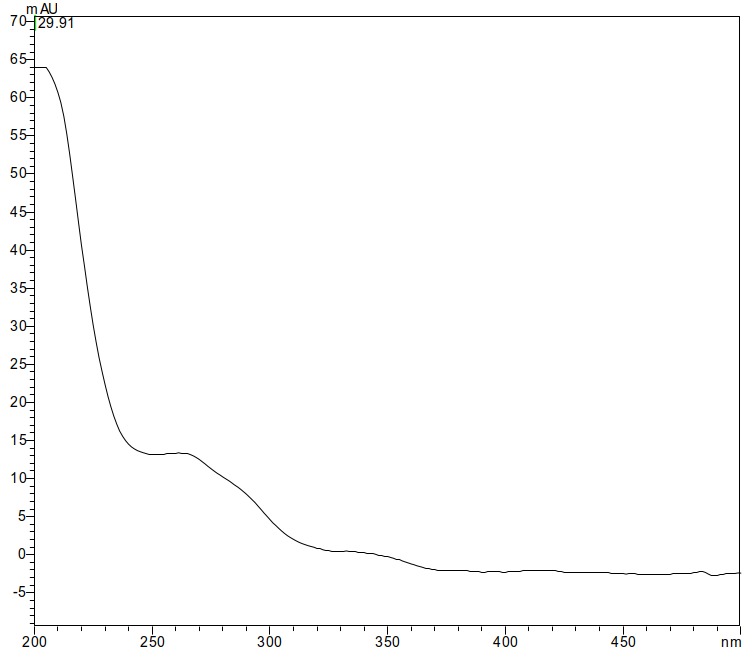
\includegraphics[width=\textwidth]{figures/Kapitel6/keineReaktion/DNCC2991.png}
    \caption{}
    \label{fig:DNCC2991}
  \end{subfigure}
  
  \begin{subfigure}[b]{0.5\textwidth}
    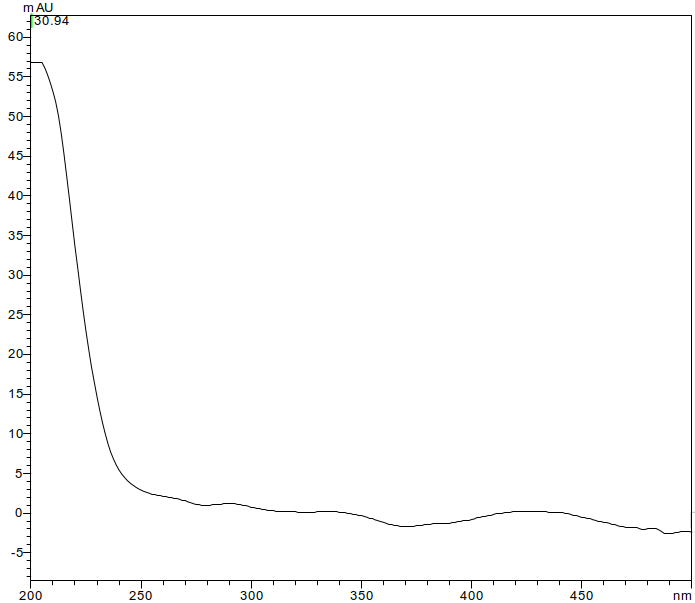
\includegraphics[width=\textwidth]{figures/Kapitel6/keineReaktion/YCC3094.png}
    \caption{}
    \label{fig:YCC3094}
  \end{subfigure}
  \caption[Online-UV/Vis Spektren mit der Charakteristik eines NCC bei 27.10 min., eines DNCC bei 29.75 min. sowie eines YCC bei 30.94 min., Quelle: Autor]{Online-UV/Vis Spektren: (a) charakteristisch für einen \gls{NCC} - RT = 27.25 min., (b) charakteristisch für einen \gls{DNCC} - RT = 29.91 min., (c) charakteristisch für einen \gls{YCC} - RT = 30.94 min.}
\end{figure}
